% Inbuilt themes in beamer
\documentclass[aspectratio=169]{beamer}
\usepackage{graphicx}
% Theme choice:
\usetheme{CambridgeUS}

% Title page details: 
\title{Chapter 7: Consumers, Producers, and the Efficiency of Markets} 
\author{Discussion section 4}
\date{October 2023}

\begin{document}

% Title page
\begin{frame}
    \titlepage 
\end{frame}

% Outline frame
\begin{frame}{Outline}
    So far we have tried to understand \textbf{how} markets work: a \textit{positive} rather than \textit{normative} project.

    \vspace{5mm}

    Now we will start to look at \textbf{welfare economics}: how well-being is effected by different market outcomes.
\end{frame}

\begin{frame}{Willingness to pay}
    Each consumer will have a different \textit{willingness to pay} for a good.
    
    \vspace{2mm}

    There is a maximum amount they will spend; at any price below this they purchase the good, and at any price above they do not.

    \vspace{2mm}

    The difference between the amount they \textit{actually} spend and the amount they are \textit{willing} to spend is their \textbf{consumer surplus}.

\end{frame}

\begin{frame}{Consumer surplus}
    Consumer surplus is the area below the demand curve and above the market price.

    \centering
    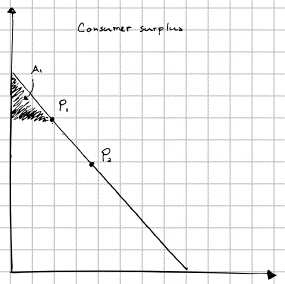
\includegraphics[width = 0.4\textwidth,keepaspectratio]{../figs/surplus1.png}

    What happens to consumer surpluse when the price moves from $P_1$ to $P_2$?
\end{frame}

\begin{frame}{Consumer surplus}
    Some benefit accrues to already participating consumers and some to new consumers.

    \centering
    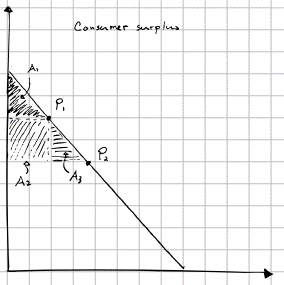
\includegraphics[width = 0.4\textwidth,keepaspectratio]{../figs/surplus2.png}
\end{frame}

\begin{frame}{Consumer surplus}
    Consumer surplus depends on willingness to pay, so how might we measure this?

    \vspace{5mm}

    Consumer surplus measures the benefit consumers' receive from a good, ``as they themselves perceive it''.
\end{frame}

\begin{frame}{Producer surplus}
    Producer surplus is essentially the same.
    
    \vspace{5mm}

    Depends on \textit{cost}: the value of everything a seller must give up to produce a good.

    \vspace{5mm}

    Given by the area above the supply curve and below the market price.
\end{frame}

\begin{frame}{Efficiency}
    A market outcome is \textit{efficient} if it maximizes the \textbf{total surplus} of producers and Consumers

    \vspace{2mm}

    Total surpluse = consumer surplus + producer surplus = value to buyers - cost to sellers

    \vspace{2mm}

    We might also care about \textit{equality}, or the distribution of surplus between producers and consumers

\end{frame}

\begin{frame}{Market for coffee}
    Let's return to our market for coffee.

    \vspace{5mm}

    Identify the area of total surplus, splitting it into consumer surplus and producer surplus.
\end{frame}

\begin{frame}{Market for coffee}
    \centering
    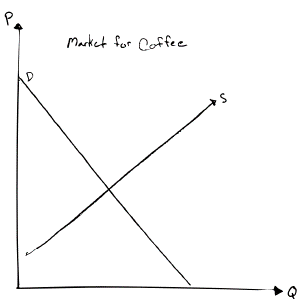
\includegraphics[width = 0.4\textwidth,keepaspectratio]{../figs/coffee1.png}
\end{frame}

\begin{frame}{Total surplus in the market for coffee}
    \centering
    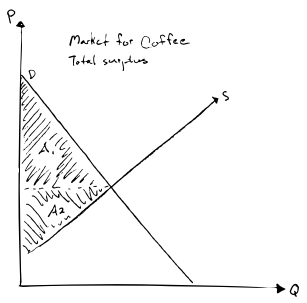
\includegraphics[width = 0.4\textwidth,keepaspectratio]{../figs/coffee2.png}
\end{frame}

\begin{frame}{Market for coffee}
    Now suppose the government imposes a tax on consumption of coffee.

    \vspace{2mm}

    \begin{enumerate}
        \item Illustrate the impact of the tax on the market equilibrium; what happens to P and Q?
        \item What happens to consumer surplus?
        \item Producer surplus?
        \item Total surplus?
    \end{enumerate}
\end{frame}

\begin{frame}{Tax on market for coffee}
    \centering
    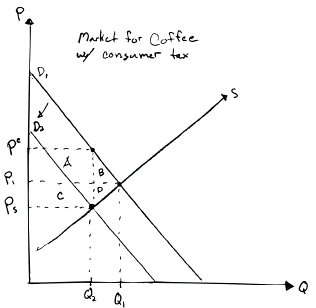
\includegraphics[width = 0.4\textwidth,keepaspectratio]{../figs/coffee4.png}
\end{frame}

\begin{frame}{Tax on market for coffee}
    The effects are:
    \begin{itemize}
        \item Consumer surplus decreases by $A + B$
        \item Producer surplus decreases by $C + D$
        \item Government revenue is given by $A + C$
        \item $(A+C) - (A+B) - (C+D) = -(B + D)$ is deadweight loss
    \end{itemize}
\end{frame}

\begin{frame}{Subsidy in market for coffee}
    Let's try something else: suppose the government provides a \textit{subsidy} to suppliers.

    \vspace{2mm}

    \begin{enumerate}
        \item Illustrate the impact of the subsidy on the market equilibrium; what happens to P and Q?
        \item What happens to consumer surplus?
        \item Producer surplus?
        \item Total surplus?
    \end{enumerate}
\end{frame}

\begin{frame}{Tax on market for coffee}
    \centering
    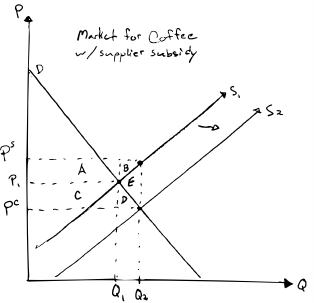
\includegraphics[width = 0.4\textwidth,keepaspectratio]{../figs/coffee3.png}
\end{frame}

\begin{frame}{Subsidy in market for coffee}
    The effects are:
    \begin{itemize}
        \item Consumer surplus increases by $C + D$
        \item Producer surplus increases by $A + B$
        \item Government spends$ A + B + C + D + E $
        \item $(C+D) + (A + B) -  (A + B + C + D + E) = - E$ is deadweight loss
    \end{itemize}
\end{frame}

\begin{frame}{Total Surplus}
    In both cases, government interventions were not able to improve the market outcome without creating deadweight loss.

    \vspace{2mm}

    In our simplistic, perfectly competitive market:
    \begin{itemize}
        \item Supply of goods go to the buyers who value them the most
        \item Demand for goods go to the producers who can make them at the lowest cost
        \item The market equilibrium thus maximizes the sum of consumer and producer surplus
    \end{itemize}
\end{frame}

\begin{frame}{Efficiency}
    Note that this tells us nothing about \textit{equality}.

    \vspace{5mm}

    In addition, we have not addressed:
    \begin{itemize}
        \item Market power
        \item Externalities
        \item Other market failures
    \end{itemize}

    And other violations of our assumptions, which might make this conclusion fail.
\end{frame}

\begin{frame}{Application}
    Let's consider the market for iPhones.

    \vspace{2mm}

    Is the demand for iPhones elastic or inelastic? What about supply?

    \vspace{2mm}

    Illustrate the impact of a decrease in the cost of production.
\end{frame}

\begin{frame}{Application}
    Let's consider the market for iPhones.

    \vspace{2mm}

    Is the demand for iPhones elastic or inelastic? What about supply?

    \vspace{2mm}

    Illustrate the impact of a decrease in the cost of production and show the change to surplus.
\end{frame}

\begin{frame}
    \frametitle{Application}
    \centering
    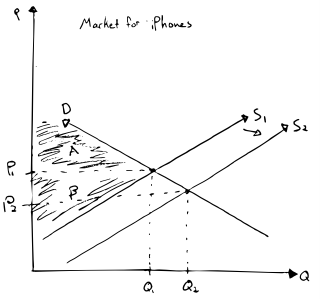
\includegraphics[width = 0.4\textwidth,keepaspectratio]{../figs/iphone1.png}
\end{frame}

\begin{frame}
    \frametitle{Application}
    \centering
    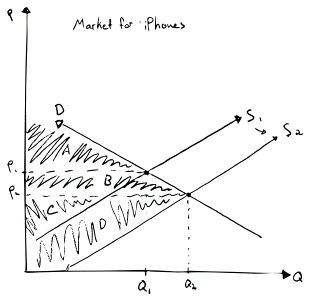
\includegraphics[width = 0.4\textwidth,keepaspectratio]{../figs/iphone2.png}
\end{frame}

\begin{frame}{Application}
    Some of the effects are:
    \begin{enumerate}
        \item New equilibrium price is lower and quantity is higher
        \item Total surplus unambiguously increases
        \item Both consumers and producers have a larger surplus than before
    \end{enumerate}
    
    I drew relatively elastic supply and demand curves; now consider if the supply was elastic, but the demand was very inelastic.
\end{frame}

\begin{frame}
    \frametitle{Application}
    \centering
    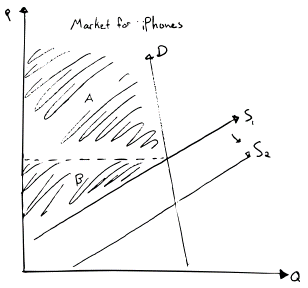
\includegraphics[width = 0.4\textwidth,keepaspectratio]{../figs/iphone3.png}
\end{frame}

\begin{frame}
    \frametitle{Application}
    \centering
    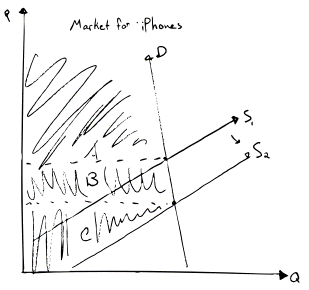
\includegraphics[width = 0.4\textwidth,keepaspectratio]{../figs/iphone4.png}
\end{frame}

\begin{frame}{Application}
    Our graph suggests that the consumer surplus increases by more than producers

    \vspace{2mm}

    This is correct! And think about the inuition: if demand is inelastic this means consumers have a very high willingness to pay, so their surplus will be large.
\end{frame}

\end{document}